%% Back matter
%
% This is where we include appendices and references
%
\appendix

\chapter{Appendix}
\section{File structure of UEC-FOOD 256}

The zip directory including all the files of the dataset contains, Fig. \ref{fig:uec_file_tree}:

\begin{figure}[h]
    \centering
    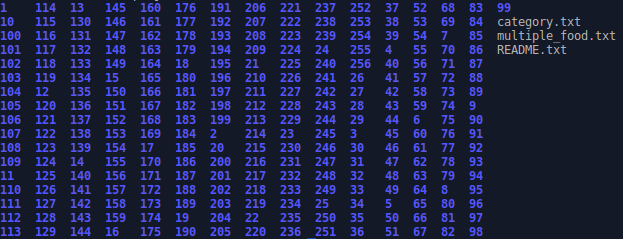
\includegraphics[scale=0.5]{img/uec_file_tree.png}
    \caption[UEC-FOOD 256 list of files and directory in the root]{UEC-FOOD 256 list of files and directory in the root. Directories are in blue, files in white.}
    \label{fig:uec_file_tree}
\end{figure}

\begin{itemize}
    \item \enquote{README}: file briefly describing the structure and including the license
    
    \item \enquote{\textbf{category.txt}}, Fig. \ref{fig:uec_file_category}: a file associating an id (a number in $[1 - 256]$) to a class, i.e. a specific food category such as rice or pizza
    
    \begin{figure}[h]
        \centering
        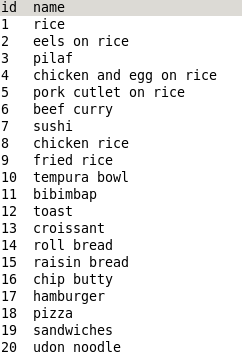
\includegraphics[scale=0.5]{img/uec_file_category.png}
        \caption[UEC-FOOD 256 file: \textit{category.txt}]{UEC-FOOD 256 file: \textit{category.txt}}
        \label{fig:uec_file_category}
    \end{figure}
    
    \item \enquote{\textbf{multiple\_food.txt}}, Fig. \ref{fig:uec_file_multiple_food}: a file giving the list of images containing multiple food categories
    
    \begin{figure}[h]
        \centering
        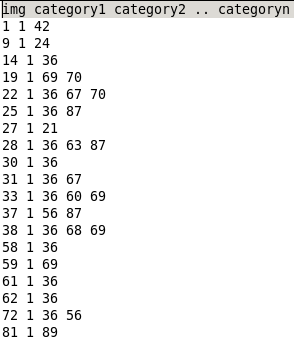
\includegraphics[scale=0.5]{img/uec_file_multiple_food.png}
        \caption[UEC-FOOD 256 file: \textit{multiple\_food.txt}]{UEC-FOOD 256 file: \textit{multiple\_food.txt}. The first column is the image filename, the following list corresponds to each class id represented on this picture.}
        \label{fig:uec_file_multiple_food}
    \end{figure}
    
    \item 256 directories, numbered from 1 to 256. Each of this directory represents a category. It includes all the pictures associated to this class. Thus, the same image can be in multiple \enquote{class category}.
    
    Moreover, each directory include a \enquote{\textbf{bb\_info.txt}}, Fig. \ref{fig:uec_file_bb_info} corresponding to the bounding box for each picture.
    
    A bounding box is represented by its coordinate as a $(x_0, y_0, x_1, y_1)$:
    \begin{itemize}
        \item $(x_0, y_0)$: coordinate of one of the point
        \item $(x_1, y_1)$: coordinate of the opposite point
    \end{itemize}
    
    \begin{figure}[h]
        \centering
        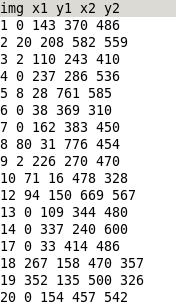
\includegraphics[scale=0.5]{img/uec_file_bb_info.png}
        \caption[UEC-FOOD 256 file: \textit{bb\_info.txt}]{UEC-FOOD 256 file: \textit{bb\_info.txt}. The first column is the image filename, the next four columns are the bounding box coordinates.}
        \label{fig:uec_file_bb_info}
    \end{figure}
\end{itemize}

\clearpage

\section{List of food categories (UEC-FOOD 256)}

UEC-FOOD 100 corresponds to the first 100 categories.

{
    % \renewcommand{\arraystretch}{1.1}
    \begin{longtable}{| c | c | c|}
        \hline
        \textbf{Food name} & \textbf{Id} & \textbf{Number of pictures} \\
        \hline
        \hline
        \endhead
        rice  &  1  &  620  \\
        \hline
        eels on rice  &  2  &  130  \\
        \hline
        pilaf  &  3  &  115  \\
        \hline
        chicken and egg on rice  &  4  &  121  \\
        \hline
        pork cutlet on rice  &  5  &  150  \\
        \hline
        beef curry  &  6  &  246  \\
        \hline
        sushi  &  7  &  153  \\
        \hline
        chicken rice  &  8  &  100  \\
        \hline
        fried rice  &  9  &  169  \\
        \hline
        tempura bowl  &  10  &  136  \\
        \hline
        bibimbap  &  11  &  112  \\
        \hline
        toast  &  12  &  218  \\
        \hline
        croissant  &  13  &  120  \\
        \hline
        roll bread  &  14  &  107  \\
        \hline
        raisin bread  &  15  &  101  \\
        \hline
        chip butty  &  16  &  148  \\
        \hline
        hamburger  &  17  &  233  \\
        \hline
        pizza  &  18  &  134  \\
        \hline
        sandwiches  &  19  &  163  \\
        \hline
        udon noodle  &  20  &  152  \\
        \hline
        tempura udon  &  21  &  106  \\
        \hline
        soba noodle  &  22  &  163  \\
        \hline
        ramen noodle  &  23  &  353  \\
        \hline
        beef noodle  &  24  &  139  \\
        \hline
        tensin noodle  &  25  &  112  \\
        \hline
        fried noodle  &  26  &  131  \\
        \hline
        spaghetti  &  27  &  151  \\
        \hline
        Japanese-style pancake  &  28  &  137  \\
        \hline
        takoyaki  &  29  &  134  \\
        \hline
        gratin  &  30  &  115  \\
        \hline
        sauteed vegetables  &  31  &  120  \\
        \hline
        croquette  &  32  &  126  \\
        \hline
        grilled eggplant  &  33  &  102  \\
        \hline
        sauteed spinach  &  34  &  102  \\
        \hline
        vegetable tempura  &  35  &  115  \\
        \hline
        miso soup  &  36  &  728  \\
        \hline
        potage  &  37  &  113  \\
        \hline
        sausage  &  38  &  118  \\
        \hline
        oden  &  39  &  112  \\
        \hline
        omelet  &  40  &  107  \\
        \hline
        ganmodoki  &  41  &  113  \\
        \hline
        jiaozi  &  42  &  167  \\
        \hline
        stew  &  43  &  106  \\
        \hline
        teriyaki grilled fish  &  44  &  105  \\
        \hline
        fried fish  &  45  &  121  \\
        \hline
        grilled salmon  &  46  &  116  \\
        \hline
        salmon meuniere  &  47  &  104  \\
        \hline
        sashimi  &  48  &  124  \\
        \hline
        grilled pacific saury  &  49  &  181  \\
        \hline
        sukiyaki  &  50  &  122  \\
        \hline
        sweet and sour pork  &  51  &  105  \\
        \hline
        lightly roasted fish  &  52  &  102  \\
        \hline
        steamed egg hotchpotch  &  53  &  108  \\
        \hline
        tempura  &  54  &  118  \\
        \hline
        fried chicken  &  55  &  154  \\
        \hline
        sirloin cutlet  &  56  &  140  \\
        \hline
        nanbanzuke  &  57  &  102  \\
        \hline
        boiled fish  &  58  &  109  \\
        \hline
        seasoned beef with potatoes  &  59  &  116  \\
        \hline
        hambarg steak  &  60  &  135  \\
        \hline
        steak  &  61  &  108  \\
        \hline
        dried fish  &  62  &  110  \\
        \hline
        ginger pork saute  &  63  &  117  \\
        \hline
        spicy chili-flavored tofu  &  64  &  120  \\
        \hline
        yakitori  &  65  &  111  \\
        \hline
        cabbage roll  &  66  &  107  \\
        \hline
        omelet  &  67  &  131  \\
        \hline
        egg sunny-side up  &  68  &  224  \\
        \hline
        natto  &  69  &  147  \\
        \hline
        cold tofu  &  70  &  158  \\
        \hline
        egg roll  &  71  &  109  \\
        \hline
        chilled noodle  &  72  &  117  \\
        \hline
        stir-fried beef and peppers  &  73  &  107  \\
        \hline
        simmered pork  &  74  &  109  \\
        \hline
        boiled chicken and vegetables  &  75  &  105  \\
        \hline
        sashimi bowl  &  76  &  147  \\
        \hline
        sushi bowl  &  77  &  111  \\
        \hline
        fish-shaped pancake with bean jam  &  78  &  122  \\
        \hline
        shrimp with chill source  &  79  &  118  \\
        \hline
        roast chicken  &  80  &  110  \\
        \hline
        steamed meat dumpling  &  81  &  115  \\
        \hline
        omelet with fried rice  &  82  &  126  \\
        \hline
        cutlet curry  &  83  &  142  \\
        \hline
        spaghetti meat sauce  &  84  &  125  \\
        \hline
        fried shrimp  &  85  &  115  \\
        \hline
        potato salad  &  86  &  128  \\
        \hline
        green salad  &  87  &  342  \\
        \hline
        macaroni salad  &  88  &  109  \\
        \hline
        Japanese tofu and vegetable chowder  &  89  &  115  \\
        \hline
        pork miso soup  &  90  &  117  \\
        \hline
        chinese soup  &  91  &  165  \\
        \hline
        beef bowl  &  92  &  167  \\
        \hline
        kinpira-style sauteed burdock  &  93  &  111  \\
        \hline
        rice ball  &  94  &  108  \\
        \hline
        pizza toast  &  95  &  105  \\
        \hline
        dipping noodles  &  96  &  126  \\
        \hline
        hot dog  &  97  &  102  \\
        \hline
        french fries  &  98  &  153  \\
        \hline
        mixed rice  &  99  &  138  \\
        \hline
        goya chanpuru  &  100  &  104  \\
        \hline
        green curry  &  101  &  100  \\
        \hline
        okinawa soba  &  102  &  108  \\
        \hline
        mango pudding  &  103  &  103  \\
        \hline
        almond jelly  &  104  &  104  \\
        \hline
        jjigae  &  105  &  107  \\
        \hline
        dak galbi  &  106  &  105  \\
        \hline
        dry curry  &  107  &  101  \\
        \hline
        kamameshi  &  108  &  101  \\
        \hline
        rice vermicelli  &  109  &  101  \\
        \hline
        paella  &  110  &  105  \\
        \hline
        tanmen  &  111  &  111  \\
        \hline
        kushikatu  &  112  &  102  \\
        \hline
        yellow curry  &  113  &  104  \\
        \hline
        pancake  &  114  &  105  \\
        \hline
        champon  &  115  &  106  \\
        \hline
        crape  &  116  &  101  \\
        \hline
        tiramisu  &  117  &  102  \\
        \hline
        waffle  &  118  &  102  \\
        \hline
        rare cheese cake  &  119  &  112  \\
        \hline
        shortcake  &  120  &  103  \\
        \hline
        chop suey  &  121  &  100  \\
        \hline
        twice cooked pork  &  122  &  113  \\
        \hline
        mushroom risotto  &  123  &  114  \\
        \hline
        namul  &  124  &  108  \\
        \hline
        zoni  &  125  &  117  \\
        \hline
        french toast  &  126  &  102  \\
        \hline
        fine white noodles  &  127  &  118  \\
        \hline
        minestrone  &  128  &  104  \\
        \hline
        pot au feu  &  129  &  114  \\
        \hline
        chicken nugget  &  130  &  103  \\
        \hline
        namero  &  131  &  111  \\
        \hline
        french bread  &  132  &  105  \\
        \hline
        rice gruel  &  133  &  116  \\
        \hline
        broiled eel bowl  &  134  &  115  \\
        \hline
        clear soup  &  135  &  115  \\
        \hline
        yudofu  &  136  &  118  \\
        \hline
        mozuku  &  137  &  101  \\
        \hline
        inarizushi  &  138  &  111  \\
        \hline
        pork loin cutlet  &  139  &  115  \\
        \hline
        pork fillet cutlet  &  140  &  115  \\
        \hline
        chicken cutlet  &  141  &  113  \\
        \hline
        ham cutlet  &  142  &  114  \\
        \hline
        minced meat cutlet  &  143  &  107  \\
        \hline
        thinly sliced raw horsemeat  &  144  &  110  \\
        \hline
        bagel  &  145  &  105  \\
        \hline
        scone  &  146  &  103  \\
        \hline
        tortilla  &  147  &  102  \\
        \hline
        tacos  &  148  &  106  \\
        \hline
        nachos  &  149  &  104  \\
        \hline
        meatloaf  &  150  &  113  \\
        \hline
        scrambled egg  &  151  &  101  \\
        \hline
        rice gratin  &  152  &  109  \\
        \hline
        lasagna  &  153  &  111  \\
        \hline
        Caesar salad  &  154  &  104  \\
        \hline
        oatmeal  &  155  &  117  \\
        \hline
        fried pork dumplings served in soup  &  156  &  116  \\
        \hline
        oshiruko or red bean soup  &  157  &  108  \\
        \hline
        muffin  &  158  &  112  \\
        \hline
        popcorn  &  159  &  116  \\
        \hline
        cream puff  &  160  &  108  \\
        \hline
        doughnut  &  161  &  112  \\
        \hline
        apple pie  &  162  &  101  \\
        \hline
        parfait  &  163  &  100  \\
        \hline
        fried pork in scoop  &  164  &  113  \\
        \hline
        lamb kebabs  &  165  &  115  \\
        \hline
        stir-fried potato and eggplant and green pepper  &  166  &  119  \\
        \hline
        roast duck  &  167  &  116  \\
        \hline
        hot pot  &  168  &  107  \\
        \hline
        pork belly  &  169  &  107  \\
        \hline
        xiao long bao  &  170  &  114  \\
        \hline
        moon cake  &  171  &  104  \\
        \hline
        custard tart  &  172  &  101  \\
        \hline
        beef noodle soup  &  173  &  118  \\
        \hline
        pork cutlet  &  174  &  103  \\
        \hline
        minced pork rice  &  175  &  111  \\
        \hline
        fish ball soup  &  176  &  119  \\
        \hline
        oyster omelette  &  177  &  102  \\
        \hline
        glutinous oil rice  &  178  &  114  \\
        \hline
        turnip pudding  &  179  &  105  \\
        \hline
        stinky tofu  &  180  &  103  \\
        \hline
        lemon fig jelly  &  181  &  109  \\
        \hline
        khao soi  &  182  &  118  \\
        \hline
        Sour prawn soup  &  183  &  108  \\
        \hline
        Thai papaya salad  &  184  &  119  \\
        \hline
        sliced Hainan-style chicken with marinated rice  &  185  &  112  \\
        \hline
        hot and sour with fish and vegetable ragout  &  186  &  111  \\
        \hline
        stir-fried mixed vegetables  &  187  &  112  \\
        \hline
        beef in oyster sauce  &  188  &  107  \\
        \hline
        pork satay  &  189  &  113  \\
        \hline
        spicy chicken salad  &  190  &  103  \\
        \hline
        noodles with fish curry  &  191  &  100  \\
        \hline
        Pork Sticky Noodles  &  192  &  120  \\
        \hline
        Pork with lemon  &  193  &  100  \\
        \hline
        stewed pork leg  &  194  &  106  \\
        \hline
        charcoal-boiled pork neck  &  195  &  115  \\
        \hline
        fried mussel pancakes  &  196  &  103  \\
        \hline
        Deep Fried Chicken Wing  &  197  &  113  \\
        \hline
        Barbecued red pork in sauce with rice  &  198  &  112  \\
        \hline
        Rice with roast duck  &  199  &  107  \\
        \hline
        Rice crispy pork  &  200  &  117  \\
        \hline
        Wonton soup  &  201  &  118  \\
        \hline
        Chicken Rice Curry With Coconut  &  202  &  104  \\
        \hline
        Crispy Noodles  &  203  &  100  \\
        \hline
        Egg Noodle In Chicken Yellow Curry  &  204  &  110  \\
        \hline
        coconut milk soup  &  205  &  111  \\
        \hline
        pho  &  206  &  117  \\
        \hline
        Hue beef rice vermicelli soup  &  207  &  114  \\
        \hline
        Vermicelli noodles with snails  &  208  &  101  \\
        \hline
        Fried spring rolls  &  209  &  104  \\
        \hline
        Steamed rice roll  &  210  &  105  \\
        \hline
        Shrimp patties  &  211  &  104  \\
        \hline
        ball shaped bun with pork  &  212  &  114  \\
        \hline
        Coconut milk-flavored crepes with shrimp and beef  &  213  &  111  \\
        \hline
        Small steamed savory rice pancake  &  214  &  106  \\
        \hline
        Glutinous Rice Balls  &  215  &  106  \\
        \hline
        loco moco  &  216  &  112  \\
        \hline
        haupia  &  217  &  103  \\
        \hline
        malasada  &  218  &  114  \\
        \hline
        laulau  &  219  &  106  \\
        \hline
        spam musubi  &  220  &  111  \\
        \hline
        oxtail soup  &  221  &  119  \\
        \hline
        adobo  &  222  &  114  \\
        \hline
        lumpia  &  223  &  110  \\
        \hline
        brownie  &  224  &  108  \\
        \hline
        churro  &  225  &  115  \\
        \hline
        jambalaya  &  226  &  109  \\
        \hline
        nasi goreng  &  227  &  110  \\
        \hline
        ayam goreng  &  228  &  103  \\
        \hline
        ayam bakar  &  229  &  114  \\
        \hline
        bubur ayam  &  230  &  108  \\
        \hline
        gulai  &  231  &  102  \\
        \hline
        laksa  &  232  &  103  \\
        \hline
        mie ayam  &  233  &  107  \\
        \hline
        mie goreng  &  234  &  104  \\
        \hline
        nasi campur  &  235  &  117  \\
        \hline
        nasi padang  &  236  &  109  \\
        \hline
        nasi uduk  &  237  &  106  \\
        \hline
        babi guling or pig roast  &  238  &  108  \\
        \hline
        kaya toast  &  239  &  114  \\
        \hline
        bak kut teh  &  240  &  107  \\
        \hline
        curry puff  &  241  &  113  \\
        \hline
        chow mein  &  242  &  116  \\
        \hline
        zha jiang mian  &  243  &  110  \\
        \hline
        kung pao chicken  &  244  &  111  \\
        \hline
        crullers  &  245  &  111  \\
        \hline
        eggplant with garlic sauce  &  246  &  113  \\
        \hline
        three cup chicken  &  247  &  117  \\
        \hline
        bean curd or tofu family style  &  248  &  105  \\
        \hline
        salt and pepper fried shrimp with shell  &  249  &  119  \\
        \hline
        baked salmon  &  250  &  109  \\
        \hline
        braised pork meat ball with napa cabbage  &  251  &  118  \\
        \hline
        winter melon soup  &  252  &  118  \\
        \hline
        steamed spareribs  &  253  &  116  \\
        \hline
        chinese pumpkin pie  &  254  &  102  \\
        \hline
        eight treasure rice  &  255  &  115  \\
        \hline
        hot and sour soup  &  256  &  117  \\
        
        \hline
         \caption{List of all the food categories of UEC-FOOD 256 with the number of pictures associated}
         \label{table:list_food}
    \end{longtable}
    %
    %
%\end{table}
}

%\section{RGB to HSV}
%
%Assuming the RGB values have been normalised to be in $[0, 1]$, we have:
%
%\begin{equation*}
%    M = \max (R, G, B)
%    \qquad
%    m = \min (R, G, B)
%    \qquad
%    C = M - m
%\end{equation*}
%
%$$
%H =
%\begin{cases}
%0 & \text{if $C = 0$}\\
%60 \times \left[ \frac{G - B}{C} \mod 6\right] & \text{if $M = R$} \\
%60 \times \left[ \frac{B - R}{C} + 2\right] & \text{if $M = G$} \\
%60 \times \left[ \frac{R - G}{C} + 4\right] & \text{if $M = B$} \\
%\end{cases}
%$$
%
%$$
%S =
%\begin{cases}
%0 & \text{if $M = 0$}\\
%\frac{C}{M}& \text{otherwise} \\
%\end{cases}
%$$
%
%$$V = M$$
%
%\section{HSV to RGB}
%
%The obtained R, G and B values are in $[0, 1]$ and calculated as such:
%
%\begin{equation*}
%    C = V \times S
%    \qquad
%    X = C \times (1 - \lvert \frac{H}{60} \mod 2 - 1\rvert )
%    \qquad
%    m = V - C
%\end{equation*}
%
%$$
%(R', G', B') = 
%\begin{cases}
%(C, X, 0) & 0 \leq H \leq 60 \\
%(X, C, 0) & 60 \leq H \leq 120 \\
%(0, C, X) & 120 \leq H \leq 180 \\
%(0, X, C) & 180 \leq H \leq 240 \\
%(X, 0, C) & 240 \leq H \leq 300 \\
%(C, 0, X) & 300 \leq H \leq 360 \\
%\end{cases}
%$$
%
%$$ (R, G, B) = (R' + m, G' + m, B' + m)$$